% This file was created with tikzplotlib v0.10.1.
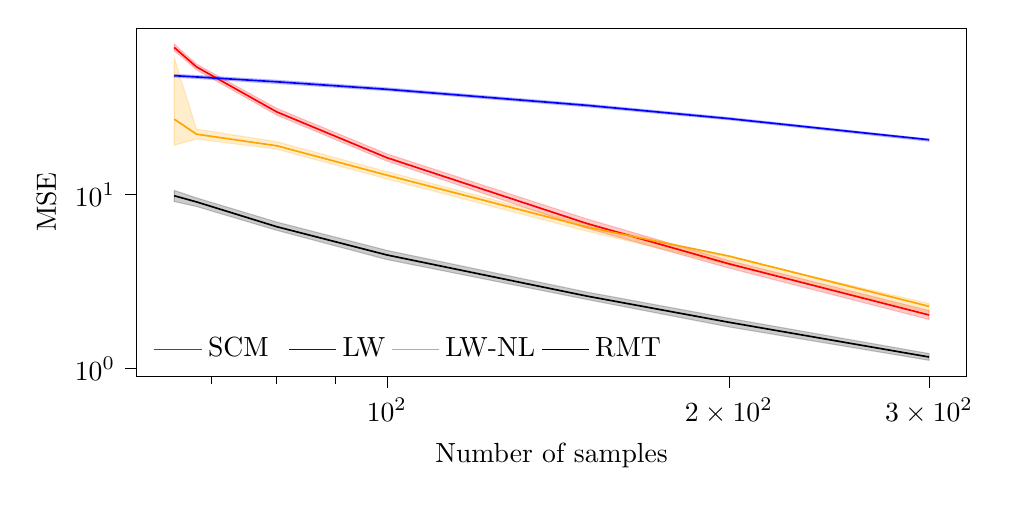
\begin{tikzpicture}

\definecolor{darkgray176}{RGB}{176,176,176}
\definecolor{green}{RGB}{0,128,0}
\definecolor{lightgray204}{RGB}{204,204,204}
\definecolor{orange}{RGB}{255,165,0}

\begin{axis}[
width=\columnwidth,
height=6cm,
legend cell align={left},
legend columns=4, 
legend style={draw=none, at={(0.01, 0.01)},anchor=south west, /tikz/column 2/.style={column sep=5pt,}},
log basis x={10},
log basis y={10},
minor xtick={2,3,4,5,6,7,8,9,20,30,40,50,60,70,80,90,200,300,400,500,600,700,800,900,2000,3000,4000,5000,6000,7000,8000,9000,20000,30000,40000,50000,60000,70000,80000,90000},
% minor xticklabels={
%   \(\displaystyle {2\times10^{0}}\),
%   \(\displaystyle {3\times10^{0}}\),
%   \(\displaystyle {4\times10^{0}}\),
%   ,
%   \(\displaystyle {6\times10^{0}}\),
%   ,
%   ,
%   ,
%   \(\displaystyle {2\times10^{1}}\),
%   \(\displaystyle {3\times10^{1}}\),
%   \(\displaystyle {4\times10^{1}}\),
%   ,
%   \(\displaystyle {6\times10^{1}}\),
%   ,
%   ,
%   ,
%   \(\displaystyle {2\times10^{2}}\),
%   \(\displaystyle {3\times10^{2}}\),
%   \(\displaystyle {4\times10^{2}}\),
%   ,
%   \(\displaystyle {6\times10^{2}}\),
%   ,
%   ,
%   ,
%   \(\displaystyle {2\times10^{3}}\),
%   \(\displaystyle {3\times10^{3}}\),
%   \(\displaystyle {4\times10^{3}}\),
%   ,
%   \(\displaystyle {6\times10^{3}}\),
%   ,
%   ,
%   ,
%   \(\displaystyle {2\times10^{4}}\),
%   \(\displaystyle {3\times10^{4}}\),
%   \(\displaystyle {4\times10^{4}}\),
%   ,
%   \(\displaystyle {6\times10^{4}}\),
%   ,
%   , 
% },
tick align=outside,
tick pos=left,
x grid style={darkgray176},
xlabel={Number of samples},
xmin=60.2147602812603, xmax=323.840864082435,
xmode=log,
xtick style={color=black},
xtick={1,10,100,200, 300, 1000,10000},
xticklabels={
  \(\displaystyle {10^{0}}\),
  \(\displaystyle {10^{1}}\),
  \(\displaystyle {10^{2}}\),
  \(\displaystyle {2\times 10^{2}}\),
  \(\displaystyle {3\times 10^{2}}\),
  \(\displaystyle {10^{3}}\),
  \(\displaystyle {10^{4}}\)
},
y grid style={darkgray176},
ylabel={MSE},
ymin=0.906831409439445, ymax=90.2554928922256,
ymode=log,
ytick style={color=black},
ytick={0.01,0.1,1,10,100,1000},
yticklabels={
  \(\displaystyle {10^{-2}}\),
  \(\displaystyle {10^{-1}}\),
  \(\displaystyle {10^{0}}\),
  \(\displaystyle {10^{1}}\),
  \(\displaystyle {10^{2}}\),
  \(\displaystyle {10^{3}}\)
}
]
\path [draw=red, fill=red, opacity=0.2]
(axis cs:65,73.2247445919917)
--(axis cs:65,67.0210988231823)
--(axis cs:68,52.12423914182)
--(axis cs:80,28.6114353039675)
--(axis cs:100,15.5891153792994)
--(axis cs:150,6.40828356957247)
--(axis cs:200,3.78637568572336)
--(axis cs:300,1.91857721931963)
--(axis cs:300,2.15837805380407)
--(axis cs:300,2.15837805380407)
--(axis cs:200,4.18032445704443)
--(axis cs:150,7.24587672600992)
--(axis cs:100,17.1466602445678)
--(axis cs:80,31.2747617984987)
--(axis cs:68,56.1631093720537)
--(axis cs:65,73.2247445919917)
--cycle;

\path [draw=blue, fill=blue, opacity=0.2]
(axis cs:65,49.0806460233759)
--(axis cs:65,47.1903059317982)
--(axis cs:68,46.4200578173441)
--(axis cs:80,43.4389546769218)
--(axis cs:100,39.5206046050163)
--(axis cs:150,31.9088267569193)
--(axis cs:200,26.8715562661357)
--(axis cs:300,20.2320580397824)
--(axis cs:300,20.8559627872577)
--(axis cs:300,20.8559627872577)
--(axis cs:200,27.7427289271786)
--(axis cs:150,33.1027747032573)
--(axis cs:100,41.0441492359144)
--(axis cs:80,45.3967295022002)
--(axis cs:68,48.3403090648444)
--(axis cs:65,49.0806460233759)
--cycle;

% \path [draw=green, fill=green, opacity=0.2]
% (axis cs:65,49.7777653993083)
% --(axis cs:65,47.8319788992543)
% --(axis cs:68,47.0386874624597)
% --(axis cs:80,43.9527265017527)
% --(axis cs:100,39.8520883909034)
% --(axis cs:150,32.1237519162816)
% --(axis cs:200,26.9943061075939)
% --(axis cs:300,20.2479584364334)
% --(axis cs:300,20.9179148262478)
% --(axis cs:300,20.9179148262478)
% --(axis cs:200,27.862191264418)
% --(axis cs:150,33.2909703469184)
% --(axis cs:100,41.3596772927665)
% --(axis cs:80,45.8730398492085)
% --(axis cs:68,49.0560000706235)
% --(axis cs:65,49.7777653993083)
% --cycle;

\path [draw=orange, fill=orange, opacity=0.2]
(axis cs:65,61.1628743156342)
--(axis cs:65,19.2140348546755)
--(axis cs:68,20.8485434640044)
--(axis cs:80,18.2332980925187)
--(axis cs:100,12.2929507734754)
--(axis cs:150,6.16176498341179)
--(axis cs:200,3.94970299030961)
--(axis cs:300,2.0989954884747)
--(axis cs:300,2.37088765165282)
--(axis cs:300,2.37088765165282)
--(axis cs:200,4.37233588203709)
--(axis cs:150,6.75169677869756)
--(axis cs:100,13.5634480543811)
--(axis cs:80,20.1356998917069)
--(axis cs:68,23.7826701552846)
--(axis cs:65,61.1628743156342)
--cycle;

\path [draw=black, fill=black, opacity=0.2]
(axis cs:65,10.5617112562306)
--(axis cs:65,9.12069655941015)
--(axis cs:68,8.548743714098)
--(axis cs:80,6.2352226578141)
--(axis cs:100,4.23591137582339)
--(axis cs:150,2.49755917576852)
--(axis cs:200,1.73886813387942)
--(axis cs:300,1.11774395779948)
--(axis cs:300,1.22238663789645)
--(axis cs:300,1.22238663789645)
--(axis cs:200,1.95026144353997)
--(axis cs:150,2.7553833244157)
--(axis cs:100,4.7841646610119)
--(axis cs:80,6.95555567484867)
--(axis cs:68,9.57450414581776)
--(axis cs:65,10.5617112562306)
--cycle;

\addplot [semithick, red]
table {%
65 69.9529340628551
68 54.1397532375746
80 29.8530930237613
100 16.2956815268801
150 6.8234209954466
200 4.00497232460151
300 2.03565650636212
};
\addlegendentry{SCM}
\addplot [semithick, blue]
table {%
65 48.1840354841978
68 47.3937130640074
80 44.4483851116391
100 40.2515744492378
150 32.5450607196298
200 27.3113782520648
300 20.6588302352151
};
\addlegendentry{LW}

\addplot [semithick, orange]
table {%
65 27.1160428106938
68 22.2422927755893
80 19.0747978732908
100 12.9294913223982
150 6.51354772616796
200 4.43829553724617
300 2.2821129477175
};
\addlegendentry{LW-NL}
\addplot [semithick, black]
table {%
65 9.84778024235454
68 9.08087941977742
80 6.5410435708147
100 4.50235050827252
150 2.61314881691979
200 1.84888784799632
300 1.16814092568788
};
\addlegendentry{RMT}
\end{axis}

\end{tikzpicture}
